\documentclass[letterpaper,10pt]{article}
\title{Assignment 3 Report - KNN and Decision Trees}
\author{Helena Bales and Natalie Suderman\\ \\ CS343 - Spring 2017}
\usepackage[pdftex]{graphicx}
\usepackage{tikz}
\usepackage{float}

\parindent = 0.0 in
\parskip = 0.1 in

\begin{document}
\maketitle

\tableofcontents
\clearpage

\section{Introduction}

\section{Model Selection for KNN}

\subsection{Implementing the K-Nearest Neighbors Algorithm}
The K-Nearest Neighbors Algorithm is implemented in Python in the file knn.py

In implementing the KNN algorithm, we first read in the datat from the provided csv. The data is 
in the form of an Nx31 dimentional matrix. The dataset constitutes 30 features with the first 
value being the true class label. For example:\\

1, 19.59, 25, 127.7, 1191, 0.1032, 0.09871, 0.1655, 0.09063, ..., 0.2293, 0.06091\\

In this case, the true class value is 1, meaning that it is malignant. If it were benign, the true
 class value would be -1.

The implementation reads in each line of the csv, removes the first value as the true class value 
then uses the following 30 features to determine the distance between data points. Before the 
distance between two points can be calculated, the scale for each feature must be determined and 
the feature scaled to be all in the same range (for example [0, 1]).

We can use the Euclidian or straight line distance to determine the distance between two points 
\(x\) and \(x_i\) with m features.

\[ x = \left[ \begin{array}{c} x_1 \\ \vdots \\ x_m \end{array} \right], x_i = \left[ \begin{array}{c} x_{i1} \\ \vdots \\ x_{im} \end{array} \right] \]
\[ D(x,x_i) = ||x - x_i|| \]
\[ D(x,x_i) = \sqrt{(x - x_i)^T(x - x_i)} \]
\[ D(x,x_i) = \sqrt{\sum_{j=1,...,m} (x_j - x_{ij})^2} \]

For each line in the csv, its k nearest neighbors will be used to determine its value.\\

\subsection{Evaluation of Error with Respect to K}
\subsubsection{Computed Training Error}
The following list are the computed training error for various \(k\) values.
\begin{itemize}
	\item{\textbf{k=1}: 0.355633802817}
	\item{\textbf{k=3}: 0.644366197183}
	\item{\textbf{k=5}: 0.355633802817 }
	\item{\textbf{k=7}: 0.355633802817}
	\item{\textbf{k=15}: 0.352112676056}
	\item{\textbf{k=21}: 0.355633802817}
	\item{\textbf{k=37}: 0.355633802817}
	\item{\textbf{k=43}: 0.355633802817}
	\item{\textbf{k=51}: 0.362676056338}
\end{itemize}
\subsubsection{Computed Leave-One-Out Cross-Validation Error}
\begin{itemize}
	\item{\textbf{k=1}: 29}
	\item{\textbf{k=3}: 22}
	\item{\textbf{k=5}: 23}
	\item{\textbf{k=7}: 27}
	\item{\textbf{k=15}: 15}
	\item{\textbf{k=21}: 24}
	\item{\textbf{k=37}: 17}
	\item{\textbf{k=43}: 21}
	\item{\textbf{k=51}: 19}
\end{itemize}
\subsubsection{Number of Errors on Provided Test Data}
\begin{itemize}
	\item{\textbf{k=1}: 183}
	\item{\textbf{k=3}: 183}
	\item{\textbf{k=5}: 101}
	\item{\textbf{k=7}: 139}
	\item{\textbf{k=15}: 101}
	\item{\textbf{k=21}: 100}
	\item{\textbf{k=37}: 151}
	\item{\textbf{k=43}: 101}
	\item{\textbf{k=51}: 100}
\end{itemize}
\subsubsection{Plot of Errors as a Function of K}
     \begin{figure}[ht]
    \centering
   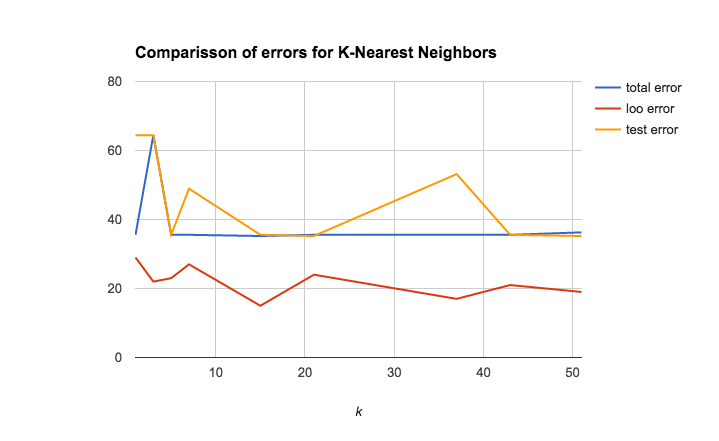
\includegraphics[width=300pt]{knn_graph.png}
    \caption{Training error, Leave-one-out Cross-validation error, and Testing error for various K values}
    \label{fig:knnError}
    \end{figure}	


\subsection{Evaluation of Different Measures of Error and Model Selection}
Based on the lecture, the leave-one-out cross-validation method of measuring error is the most informative. Given this, we should make the decision of which k value to use based on all three of the error values, however we should consider the leave-one-out error to be the most important.

From looking at the graph we can see that the lowest point in the leave-one-out error occurs when \(k = 15\). At this point, the leave-one-out error is at its global minimum of 15 and the training and testing errors are at their local minimum values of approximately 35. Given this, we should select k to be 15.

\section{Decision Tree}
\subsection{Implementing Learning Decision Tree Stump}
Best feature: 23
Best Split value: 100.25
Information Gain: .4272
Error: .3556
Test Error: .3908 
Base Branch Label: -1.0
Left Branch Label: -1.0
Right Branch Label: 1.0
\subsection{Implementing Top-Down Greedy Induction for Learning Decision Tree}

Total training error: \newline
0.557802806034 \newline
Total testing error: \newline
0.645376637757 \newline

Since the decision tree is built using the training data, it makes sense that the test data would not be as fit to the decision tree, as the training data is.  

Learned Decision Tree: \newline
values are ordered: best feature, split value, and direction of split, and class the node/branch belongs to.  
     \begin{figure}[ht]
    \centering
   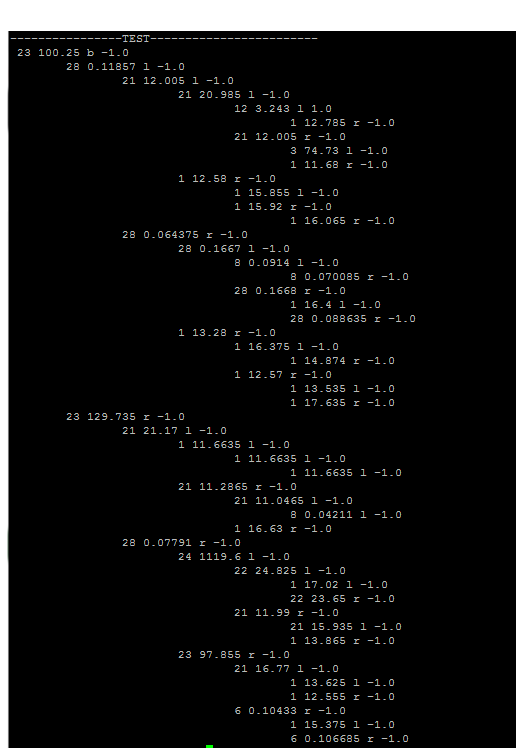
\includegraphics[width=300pt]{decisiontree.png}
    \caption{Learned decision tree}
    \label{fig:decisionTree}
    \end{figure}	


\end{document}
